\title{Study Guide for Midterm 2}
\author{Dr. Jordan Hanson - Whittier College Dept. of Physics and Astronomy}
\date{\today}
\documentclass[10pt]{article}
\usepackage[a4paper, total={18cm, 27cm}]{geometry}
\usepackage{outlines}
\usepackage{graphicx}
\begin{document}
\maketitle

\section{Memory Bank}

\begin{enumerate}
\item $\vec{F} = k \frac{q_1 q_2}{r^2}\hat{r}$ ... Coulomb Force
\item $k = 9 \times 10^{9}$ N C$^{-2}$ m$^{2}$ ... Remember $k = 1/(4\pi \epsilon_0)$.
\item $q_e = 1.6 \times 10^{-19}$ C ... Charge of an electron/proton
\item $\vec{F} = q \vec{E}$ ... Electric field and charge
\item $\vec{E}(z) = \frac{\sigma}{\epsilon_0}\hat{z}$ ... Electric field of two oppositely charge planes each with charge density $\sigma$
\item $\epsilon_0 \approx 8.85 \times 10^{-12}$ F/m
\item $dE = \int k dq / r^2$ ... Remember that $dq$ takes the form below
\item $dq = \lambda dx$ ... Linear charge density (C/m)
\item $\vec{E} \cdot \vec{A} = Q_{enc}/\epsilon_0$ ... Gauss' Law, constant electric field over the surface area.
\item $U = q\Delta V$ ... Potential energy and voltage
\item 1 eV: an electron-Volt is the amount of energy one electron gains through 1 V.
\item $V(r) = k\frac{q}{r}$ ... Voltage of a point charge
\item $\vec{E} = -\frac{\Delta V}{\Delta x}$ ... E-field is the slope or change in voltage with respect to distance
\item $V(x) = -E x + V_0$ ... Voltage is linear between two charge planes
\item $Q = CV$ ... Definition of capacitance
\item $C = \frac{\epsilon_0 A}{d}$ ... Capacitance of a parallel plate capacitor
\item $C_{tot}^{-1} = C_1^{-1} + C_2^{-1}$ ... Adding two capacitors \textit{in series.}
\item $C_{tot} = C_1 + C_2$ ... Adding two capacitors \textit{in parallel.}
\item $i(t) = dQ/dt$ ... Definition of current.
\item $v_d = i/(nqA)$ ... Charge drift velocity in a current $i$ in a conductor with number density $n$ and area $A$.
\item $R_{tot}^{-1} = R_1^{-1} + R_2^{-1}$ ... Adding two capacitors \textit{in parallel.}
\item $R_{tot} = R_1 + R_2$ ... Adding two capacitors \textit{in series.}
\item $\Delta V = I R_{\rm tot}$, $\vec{J} = \sigma \vec{E}$ ... Versions of Ohm's Law. ($\vec{J}$ is the current density with units of Amps per meter-squared).
\item $P = I V$ ... Relationship between power, current, and voltage.
\item $V_{\rm C}(t) = \epsilon_1 \left(1 - \exp(-t/\tau)\right)$ ... voltage across the capacitor in an RC series circuit.  The time constant $\tau = RC$.
\item $i(t) = \frac{\epsilon_1}{R} \exp(-t/\tau)$ ... Current in an RC series circuit.
\item $i_{\rm in} = i_{\rm out}$ ... Kirchhoff's junction rule.
\item $\epsilon_1 + \epsilon_2 + \epsilon_3 + ... = 0$ ... Kirchhoff's loop rule.
\item $\vec{F} = a\vec{v} \times \vec{B}$ ... The Lorentz force on a charge $q$ with velocity $\vec{v}$ in a magnetic field $\vec{B}$.
\item $\vec{F} = I\vec{L} \times \vec{B}$ ... The Lorentz force on a conductor of length $\vec{L}$ carrying a current $I$ in a magnetic field $\vec{B}$.
\end{enumerate}

\clearpage

\section{Chapter 9: Current and Resistance}

\begin{figure}[ht]
\centering
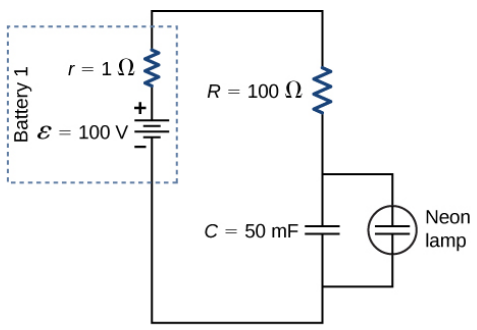
\includegraphics[width=0.3\textwidth]{circuit3.png}
\caption{\label{fig:circuit3} This type of circuit is called a relaxation oscillator.}
\end{figure}

\begin{enumerate}
\item Fig. \ref{fig:circuit3} shows a \textit{relaxation oscillator.}  The RC circuit charges, and once the capacitor voltage reaches 50 V, the neon lamp activates and completely discharges the capacitor.  The process then repeats.  Let $\tau = RC$.  We can show that the voltage across the capacitor as a function of time is
\begin{equation}
V_C(t) = \epsilon \left(1-\exp(-t/\tau)\right)
\end{equation} 
(a) How long after the circuit is connected to the battery does the neon light flash?  In other words, when is $V_C = 50$ V?  (b) What is the current initially?  (c) What is the current after a time $t >> \tau$?  \textit{By the way, it's true that $RC$ has units of time.} \\ \vspace{3cm}
\item Imagine an \textit{alternating current} (AC) system, as opposed to the DC systems we normally consider.  In AC circuits, the voltage follows a form
\begin{equation}
V(t) = V_0 \sin(2\pi f t + \phi)
\end{equation}
The wall outlets in the USA have $f = 60$ Hz and $V_0 = 120$ V.  \textit{We have the freedom to choose $\phi$ in this example, much like choosing the zero-point of voltage.}  (a) If a $5$ k$\Omega$ resistor is placed across this voltage, what will the maxium current be?  (b) What is the maximum power in the resistor?  (c) Another way to write power is $P = V^2 / R$.  What is the power consumed by the resistor 100 ms after being connected?  \\ \vspace{2cm} 
\item Three identical resistors $R$ are connected \textit{in parallel}, and powered by an adjustable voltage source. The voltage and \textit{total current} measurements are shown below. Determine the value of $R$.
\end{enumerate}

\begin{figure}[hb]
\centering
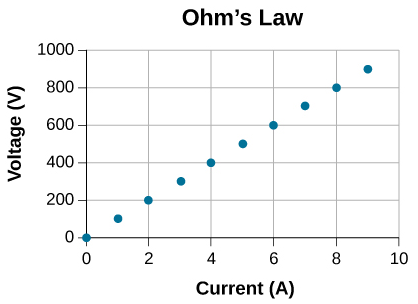
\includegraphics[width=0.33\textwidth]{ohm1.png}
\caption{\label{fig:ohm1} A graph of voltage versus current.}
\end{figure}

\clearpage

\section{Chapter 10: Direct-Current (DC) Circuits}

\begin{figure}[ht]
\centering
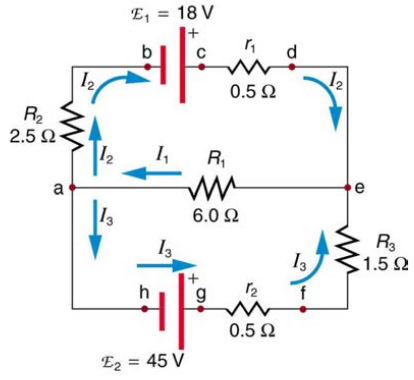
\includegraphics[width=0.4\textwidth]{circuit1.png}
\caption{\label{fig:circuit1} A circuit with two batteries and three resistors.}
\end{figure}

\begin{enumerate}
\item Solve for the current through each of the three resistors in Fig. \ref{fig:circuit1}. \\ \vspace{4cm}
\item Suppose a calculator with total resistance $R$ needs between 2.5 and 3.3 volts to operator.  Two AA batteries with $\epsilon = 1.5$V and $r = 0.25\Omega$ are connected (Fig. \ref{fig:ohm2}) in series to form a $\epsilon = 3.0$ V battery.  (a) If the calculator has an effect resistance of $R = 50\Omega$, what is the current flow? (b) If the batteries each have a charge $q = 2.5$ A hr, how long will the current flow? \\ \vspace{3cm}
\end{enumerate}

\begin{figure}[hb]
\centering
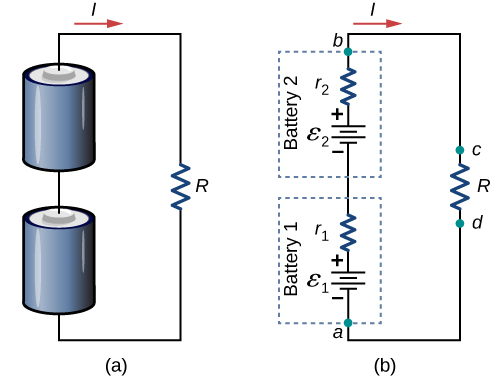
\includegraphics[width=0.35\textwidth]{ohm2.png}
\caption{\label{fig:ohm2} Two AA batteries are connected \textit{in series} to power a calculator represented by $R$.  (a) The batteries are connected in series.  (b) A circuit diagram representing the circuit in (a).}
\end{figure}

\clearpage

\section{Chapter 11: Magnetic Forces and Fields}

\begin{figure}[ht]
\centering
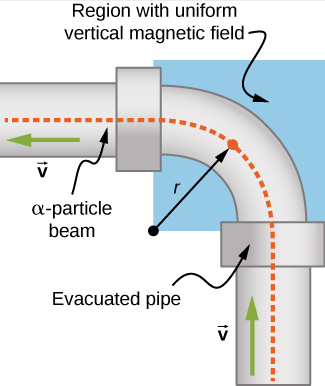
\includegraphics[width=0.25\textwidth]{pipe1.png}
\caption{\label{fig:pipe1} The trajectory of a beam of alpha-particles with $m = 6.64 \times 10^{-27}$ kg and charge $q = 3.2 \times 10^{-19}$ C is curved 90 degrees to the left.}
\end{figure}


\begin{enumerate}
\item \textbf{Practice with cross-products.}  Evaluate the following cross-products:
\begin{itemize}
\item $\vec{v}_1 = 4\hat{i}+4\hat{j}$, $\vec{v}_2 = -2\hat{i}-2\hat{j}$.  $\vec{v}_1 \times \vec{v}_2 = $
\item $\vec{v}_1 = 4\hat{i}-4\hat{j}$, $\vec{v}_2 = 2\hat{i}-2\hat{j}$.  $\vec{v}_1 \times \vec{v}_2 = $
\item $\vec{v}_1 = -2\hat{i}+2\hat{j}$, $\vec{v}_2 = -3\hat{i}+2\hat{j}$.  $\vec{v}_1 \times \vec{v}_2 = $
\item $\vec{v}_1 = -2\hat{i}-2\hat{j}+\hat{k}$, $\vec{v}_2 = 3\hat{i}+2\hat{j}-\hat{k}$.  $\vec{v}_1 \times \vec{v}_2 = $
\end{itemize} \vspace{3cm}
\item A research group is investigating short-lived radioactive isotopes. They need to design a way to transport alpha-particles (helium nuclei) from where they are made to a place where they will collide with another material to form an isotope. The alpha-particles form a beam (Fig. \ref{fig:pipe1}) that bends through a 90-degree region with a uniform magnetic field of 0.050 T. (a) In what direction should the magnetic field be applied? (b) Suppose the radius of curvature is 1.0 meter.  What is the velocity of the alpha particles?  \textit{Hint: think about how the Lorentz force must provide the centripetal force.}
\end{enumerate}

\end{document}